\documentclass[11pt]{article}

% ==========================================================
% GLOBAL PACKAGES + CONFIG (EB)
% ==========================================================
% ==========================================================
% macros/packages.tex
% Electric Barometer (EB) — Global Packages
%
% Intent:
% - Centralize shared package imports and common configuration.
% - Keep ordering consistent across documents.
% - This file includes hyperref LAST. Do not load additional packages after
%   inputting this file in your main.tex.
% ==========================================================

% ----------------------------------------------------------
% Core typography & encoding
% ----------------------------------------------------------
\usepackage[T1]{fontenc}
\usepackage[utf8]{inputenc}
\usepackage{lmodern}

% ----------------------------------------------------------
% Page layout
% ----------------------------------------------------------
\usepackage[margin=1in]{geometry}

% ----------------------------------------------------------
% Mathematics
% ----------------------------------------------------------
\usepackage{amsmath}
\usepackage{amsfonts}
\usepackage{amssymb}

% ----------------------------------------------------------
% Tables & figures
% ----------------------------------------------------------
\usepackage{graphicx}
\usepackage{booktabs}

% Common utilities used across notes/papers
\usepackage{xcolor}
\usepackage{enumitem}

% Table helpers (used in some notes)
\usepackage{adjustbox}
\usepackage{tabularx}

% ----------------------------------------------------------
% TikZ & PGFPlots (standardized across EB)
% ----------------------------------------------------------
\usepackage{tikz}
\usetikzlibrary{
  arrows.meta,
  positioning,
  shapes.geometric,
  fit,
  calc,
  backgrounds,
  intersections
}

\usepackage{pgfplots}
\pgfplotsset{compat=1.18}
\usepgfplotslibrary{
  groupplots,
  fillbetween
}

% ----------------------------------------------------------
% Formatting utilities (used in multiple notes/papers)
% ----------------------------------------------------------
\usepackage{framed}
\usepackage{setspace}

% ----------------------------------------------------------
% Citations
% ----------------------------------------------------------
\usepackage[authoryear,round]{natbib}

% ----------------------------------------------------------
% Microtypography
% ----------------------------------------------------------
\usepackage{microtype}

% ----------------------------------------------------------
% Hyperlinks (MUST be loaded last)
% ----------------------------------------------------------
\usepackage[hidelinks]{hyperref}


% ==========================================================
% CUSTOM MACROS (shared notation)
% ==========================================================
% ==========================================================
% EB-PAPERS: CANONICAL MACROS / COMMANDS
% Forecast Readiness Framework (FRF) / Electric Barometer
% ==========================================================
% Goals:
% - One meaning per symbol.
% - Shared across all papers/notes/briefs.
% - Backwards-compatible aliases.
% - Avoid redefinition errors via \providecommand.
% ==========================================================

% ----------------------------------------------------------
% Core framework / artifacts
% ----------------------------------------------------------
\providecommand{\FRF}{\ensuremath{\mathrm{FRF}}}
\providecommand{\FRS}{\ensuremath{\mathrm{FRS}}}

\providecommand{\FPC}{\ensuremath{\mathrm{FPC}}}
\providecommand{\DQC}{\ensuremath{\mathrm{DQC}}}
\providecommand{\Governance}{\ensuremath{\mathrm{Governance}}}
\providecommand{\GovernanceDecision}{\ensuremath{\mathrm{GovernanceDecision}}}

\providecommand{\RAL}{\ensuremath{\mathrm{RAL}}}

% Readiness primitives / governance vocabulary
\providecommand{\ReadinessPrimitive}{\ensuremath{\mathrm{RP}}}

% Limited-Time Offers
\providecommand{\LTO}{\ensuremath{\mathrm{LTO}}}
\providecommand{\LTOs}{\ensuremath{\mathrm{LTOs}}}

% ----------------------------------------------------------
% Core metrics (upright math)
% ----------------------------------------------------------
\providecommand{\CWSL}{\ensuremath{\mathrm{CWSL}}}
\providecommand{\CWSLR}{\ensuremath{\mathrm{CWSLR}}} % named artifact in prose
\providecommand{\NSL}{\ensuremath{\mathrm{NSL}}}
\providecommand{\UD}{\ensuremath{\mathrm{UD}}}
\providecommand{\HR}{\ensuremath{\mathrm{HR}}}
\providecommand{\HRtau}{\ensuremath{\mathrm{HR}@\tau}}

% FRS sub-terms
\providecommand{\CWSLscaled}{\ensuremath{\mathrm{CWSL}_{\mathrm{scaled}}}}
\providecommand{\CWSLmax}{\ensuremath{\mathrm{CWSL}_{\max}}}

% Legacy HR macro names
\providecommand{\HRAT}{\ensuremath{\mathrm{HR@\tau}}}
\providecommand{\tauTol}{\ensuremath{\tau}}
\providecommand{\tauop}{\ensuremath{\tau}}

% ----------------------------------------------------------
% Indexing and sets
% ----------------------------------------------------------
\providecommand{\Iset}{\ensuremath{I}}
\providecommand{\Tset}{\ensuremath{T}}

\providecommand{\entity}{\ensuremath{i}}
\providecommand{\timeindex}{\ensuremath{t}}

% Back-compat index shorthands
\providecommand{\iidx}{\entity}
\providecommand{\tidx}{\timeindex}

% Summation shorthand
\providecommand{\sumit}{\ensuremath{\sum_{\entity \in \Iset} \sum_{\timeindex \in \Tset}}}

% Optional sizes / counts
\providecommand{\Tsize}{\ensuremath{|\Tset|}}
\providecommand{\nobs}{\ensuremath{N}}

% ----------------------------------------------------------
% Forecast / demand notation
% ----------------------------------------------------------
\providecommand{\y}{\ensuremath{y}}
\providecommand{\yhat}{\ensuremath{\hat{y}}}

\providecommand{\yit}{\ensuremath{y_{\entity\timeindex}}}
\providecommand{\yhatit}{\ensuremath{\hat{y}_{\entity\timeindex}}}

% Common residuals / errors
\providecommand{\errit}{\ensuremath{e_{\entity\timeindex}}}
\providecommand{\resit}{\errit} % alias
\providecommand{\absit}{\ensuremath{\left|\yhatit - \yit\right|}}
\providecommand{\abserrit}{\absit} % alias

% Explicit residual definition macro (optional)
\providecommand{\resdef}{\ensuremath{\errit = \yit - \yhatit}}

% ----------------------------------------------------------
% Shortfall / overbuild decomposition
% ----------------------------------------------------------
\providecommand{\shortfall}{\ensuremath{s}}
\providecommand{\overbuild}{\ensuremath{o}}

\providecommand{\sit}{\ensuremath{s_{\entity\timeindex}}}
\providecommand{\oit}{\ensuremath{o_{\entity\timeindex}}}

% Positive-part operator (canonical name)
\providecommand{\pospart}[1]{\left(#1\right)_{+}}

% Explicit decompositions
\providecommand{\shortfalldef}{\ensuremath{\sit = \pospart{\yit - \yhatit}}}
\providecommand{\overbuilddef}{\ensuremath{\oit = \pospart{\yhatit - \yit}}}

% Back-compat convenience symbols used in some notes
\providecommand{\sdepth}{\shortfall} % UD paper convenience

% ----------------------------------------------------------
% Indicators / expectations / operators
% ----------------------------------------------------------
% Canonical indicator: \Ind{event}
\providecommand{\Ind}{\ensuremath{\mathbb{I}}}
\providecommand{\indicator}[1]{\ensuremath{\mathbf{1}\{#1\}}} % prose-friendly alternative

% Back-compat: some notes used \Indicator (capital I). Keep as an alias to the
% canonical \Ind to avoid duplicate meanings.
\providecommand{\Indicator}{\Ind}

% If you want function-style indicator without braces: \Ind\!(event)
% Keep as \Ind and let authors decide.
\providecommand{\E}{\ensuremath{\mathbb{E}}}

\providecommand{\abs}[1]{\left|#1\right|}
\providecommand{\card}[1]{\left|#1\right|}

% ----------------------------------------------------------
% Cost parameters + cost ratio calibration (CWSLR note)
% ----------------------------------------------------------
% IMPORTANT: Canonical costs are subscripted (c_u, c_o). This avoids
% collisions with superscript variants.
\providecommand{\cu}{\ensuremath{c_u}}
\providecommand{\co}{\ensuremath{c_o}}

% Entity-specific costs
\providecommand{\cui}{\ensuremath{c_{u,\entity}}}
\providecommand{\coi}{\ensuremath{c_{o,\entity}}}

% Cost ratio
\providecommand{\R}{\ensuremath{R}}
\providecommand{\Ri}{\ensuremath{R_{\entity}}}
\providecommand{\Rdef}{\ensuremath{R = \cu/\co}}

% Aggregate under/over cost functions (used in calibration prose)
\providecommand{\UnderCost}{\ensuremath{\mathrm{UnderCost}}}
\providecommand{\OverCost}{\ensuremath{\mathrm{OverCost}}}

% Candidate grid
\providecommand{\Rgrid}{\ensuremath{\mathcal{R}}}

% Calibrated selections
\providecommand{\Rstar}{\ensuremath{R^{\ast}}}
\providecommand{\Rist}{\ensuremath{R^{\ast}_{\entity}}}

% CWSL as a function of R (notation)
\providecommand{\CWSLofR}{\ensuremath{\CWSL(\R)}}
\providecommand{\CWSLofRi}{\ensuremath{\CWSL(\Ri)}}

% Balance-based selection operator (kept as a macro because you used it)
\providecommand{\Rbalance}{%
\ensuremath{%
\arg\min_{\R \in \Rgrid}\left|\UnderCost(\R) - \OverCost(\R)\right|%
}%
}

% Back-compat (older notes used superscripts c^u / c^o)
\providecommand{\cuSup}{\ensuremath{c^{u}}}
\providecommand{\coSup}{\ensuremath{c^{o}}}
\providecommand{\cuiSup}{\ensuremath{c^{u}_{\entity}}}
\providecommand{\coiSup}{\ensuremath{c^{o}_{\entity}}}

% ----------------------------------------------------------
% HR@tau scanning / calibration (HRtau note)
% ----------------------------------------------------------
\providecommand{\tauval}{\ensuremath{\tau}}
\providecommand{\tauv}{\tauval}
\providecommand{\taui}{\ensuremath{\tau_{\entity}}}

% Candidate tolerance grid
\providecommand{\TauGrid}{\ensuremath{\mathcal{T}}}

% Calibrated tolerances
\providecommand{\taustar}{\ensuremath{\tau^{\ast}}}
\providecommand{\taustari}{\ensuremath{\tau^{\ast}_{\entity}}}

% Target hit-rate (if used)
\providecommand{\hstar}{\ensuremath{h^{\ast}}}

% Hit indicator definition helpers
\providecommand{\Hitit}{\ensuremath{h_{\entity\timeindex}}}
\providecommand{\HitDef}{\ensuremath{\Hitit = \Ind\!\left(\absit \le \tauval\right)}}

% HR as a function of tau
\providecommand{\HRoftau}{\ensuremath{\HR(\tauval)}}
\providecommand{\HRtauoftau}{\ensuremath{\HRtau(\tauval)}}

% Optional utility selection helpers
\providecommand{\lambdau}{\ensuremath{\lambda}}
\providecommand{\taumax}{\ensuremath{\tau_{\max}}}
\providecommand{\Utility}{\ensuremath{\mathcal{U}}}
\providecommand{\UtilityDef}{\ensuremath{\Utility(\tauval) = \HR(\tauval) - \lambdau \cdot (\tauval/\taumax)}}

% Governance guards
\providecommand{\taufloor}{\ensuremath{\tau_{\min}}}
\providecommand{\taucap}{\ensuremath{\tau_{\mathrm{cap}}}}
\providecommand{\nmin}{\ensuremath{n_{\min}}}

% ----------------------------------------------------------
% DQC / snapping / quantization (DQC note)
% ----------------------------------------------------------
\providecommand{\gunit}{\ensuremath{g}}
\providecommand{\guniti}{\ensuremath{g_{\entity}}}

\providecommand{\ygrid}{\ensuremath{\tilde{y}}}
\providecommand{\ygridit}{\ensuremath{\tilde{y}_{\entity\timeindex}}}

\providecommand{\yhatgrid}{\ensuremath{\tilde{\hat{y}}}}
\providecommand{\yhatgridit}{\ensuremath{\tilde{\hat{y}}_{\entity\timeindex}}}

\providecommand{\snap}{\ensuremath{\mathcal{S}}}
\providecommand{\snaphatdef}{\ensuremath{\yhatgridit = \snap_{\gunit}\!\left(\yhatit\right)}}
\providecommand{\snapydef}{\ensuremath{\ygridit = \snap_{\gunit}\!\left(\yit\right)}}

\providecommand{\residit}{\ensuremath{r_{\entity\timeindex}}}
\providecommand{\residdef}{\ensuremath{\residit = \yit - \ygridit}}

\providecommand{\MAD}{\ensuremath{\mathrm{MAD}}}
\providecommand{\IQR}{\ensuremath{\mathrm{IQR}}}

\providecommand{\multirate}{\ensuremath{\rho}}
\providecommand{\multiratei}{\ensuremath{\rho_{\entity}}}

\providecommand{\DeltaStar}{\ensuremath{\Delta^{\ast}}}

\providecommand{\Pset}{\ensuremath{\mathcal{P}}}
\providecommand{\packunit}{\ensuremath{p}}
\providecommand{\packuniti}{\ensuremath{p_{\entity}}}

% DQC classes
\providecommand{\ContinuousLike}{\textsc{Continuous-like}}
\providecommand{\Quantized}{\textsc{Quantized}}
\providecommand{\PiecewisePacked}{\textsc{Piecewise-packed}}

% FPC classes
\providecommand{\Compatible}{\textsc{Compatible}}
\providecommand{\Marginal}{\textsc{Marginal}}
\providecommand{\Incompatible}{\textsc{Incompatible}}

% ----------------------------------------------------------
% RAL shorthands used in notes
% ----------------------------------------------------------
\providecommand{\alphaadj}{\ensuremath{\alpha}}

% RAL operator (functional form)
\providecommand{\RALop}{\ensuremath{\mathcal{R}_{\alphaadj}}}

\providecommand{\yhatadjit}{\ensuremath{\hat{y}^{(\alphaadj)}_{\entity\timeindex}}}
\providecommand{\yhatadjdef}{\ensuremath{\yhatadjit = (1+\alphaadj)\,\yhatit}}

\providecommand{\dNSL}{\ensuremath{\Delta \NSL}}
\providecommand{\dHRtau}{\ensuremath{\Delta \HRtau}}
\providecommand{\dCWSL}{\ensuremath{\Delta \CWSL}}

% ----------------------------------------------------------
% Governance policy handles
% ----------------------------------------------------------
\providecommand{\TauPolicy}{\ensuremath{\mathrm{TauPolicy}}}
\providecommand{\RALPolicy}{\ensuremath{\mathrm{RALPolicy}}}
\providecommand{\UnitPolicy}{\ensuremath{\mathrm{UnitPolicy}}}

\providecommand{\GovernanceStatus}{\ensuremath{\mathrm{GovernanceStatus}}}
\providecommand{\Green}{\textsc{Green}}
\providecommand{\Yellow}{\textsc{Yellow}}
\providecommand{\Red}{\textsc{Red}}

\providecommand{\RawUnits}{\textsc{Raw}}
\providecommand{\SnappedUnits}{\textsc{Snapped}}

% ----------------------------------------------------------
% LTO paper specifics
% ----------------------------------------------------------
\providecommand{\ltoOn}{\ensuremath{z_{\timeindex}}}
\providecommand{\ltoPhase}{\ensuremath{\phi_{\timeindex}}}
\providecommand{\qprod}{\ensuremath{\mathrm{QP}}}

% ----------------------------------------------------------
% Frontmatter helpers
% ----------------------------------------------------------
\providecommand{\keywords}[1]{%
\par\noindent\textbf{Keywords: }#1\par
}

% ----------------------------------------------------------
% Prose shorthands
% ----------------------------------------------------------
\providecommand{\ie}{i.e.\ }
\providecommand{\eg}{e.g.\ }

% ==========================================================
% END
% ==========================================================


% ==========================================================
% STYLE LAYER (EB)
% ==========================================================
% ==========================================================
% macros/style.tex
% Electric Barometer — Style Layer (v1)
% ----------------------------------------------------------
% Scope (v1):
%   - PDF metadata only
%
% Notes:
%   - Assumes hyperref is already loaded via macros/packages.tex
%   - This file should NOT load packages.
% ==========================================================

% ----------------------------------------------------------
% PDF METADATA (canonical helper)
% ----------------------------------------------------------
% Usage:
%   \EBPdfMeta{<pdftitle>}{<pdfauthor>}{<pdfsubject>}{<pdfkeywords>}
%
% Examples:
%   \EBPdfMeta
%     {Cost-Weighted Service Loss (CWSL): An Asymmetric Cost Metric for Forecast Evaluation}
%     {Kyle Corrie}
%     {Technical Note — Electric Barometer Series}
%     {Electric Barometer, Forecast Readiness Framework, CWSL, asymmetric loss}
%
\newcommand{\EBPdfMeta}[4]{%
  \hypersetup{%
    pdftitle={#1},%
    pdfauthor={#2},%
    pdfsubject={#3},%
    pdfkeywords={#4},%
    colorlinks=true,%
    linkcolor=blue,%
    citecolor=blue,%
    urlcolor=blue%
  }%
}


% ==========================================================
% PDF METADATA
% ==========================================================
% NOTE: \EBPdfMeta is defined in ../../macros/style.tex. In the EB stack it is
% commonly a 3-argument helper (Title, Author, Keywords). Providing the third
% argument prevents runaway-argument failures if the macro expects it.
%
% IMPORTANT: Keep this call on a single paragraph (no blank lines inside any
% macro argument). If you ever need line breaks, use % at end-of-line.
\EBPdfMeta{Managing Limited-Time Offers under Forecast Uncertainty: A Readiness-Centric Approach to Production Management}{Kyle Corrie}{limited-time offers, production management, operational forecasting, readiness, asymmetric loss, governance}

% ==========================================================
% DOCUMENT
% ==========================================================
\begin{document}

% ==========================================================
% FRONTMATTER
% ==========================================================
\title{The Forecast Readiness Framework: Evaluating Asymmetric Forecast Performance in Operational Systems}

\author{
  Kyle Corrie\\[6pt]
  \small Forecast Readiness Framework (FRF)\\
  \small Electric Barometer Series
}

\date{}

\maketitle

\begin{abstract}
Forecast performance in operational environments is commonly evaluated using symmetric
accuracy metrics such as MAE, RMSE, and MAPE. These measures implicitly assume that
over-forecasting and under-forecasting impose equivalent cost, an assumption that rarely holds
in high-frequency systems where shortages generate substantially greater operational disruption
than excess. As a result, forecasts that appear accurate by traditional metrics may still fail to
support reliable execution.

We introduce the \emph{Forecast Readiness Framework} (FRF), a multi-dimensional approach
for evaluating forecast performance under asymmetric error structures. Rather than relying on
a single loss function, the framework decomposes readiness into complementary dimensions
capturing service reliability, failure severity, tolerance stability, and economic consequence.
Within this framework, Cost-Weighted Service Loss (CWSL) serves as the primary economic
axis, explicitly quantifying the asymmetric operational impact of forecast error, while supporting
diagnostics characterize how frequently shortfalls occur, how severe they are when they arise,
and whether deviations fall within operationally absorbable bounds.

By reframing forecast evaluation around readiness for deployment rather than numerical accuracy
alone, the Forecast Readiness Framework provides a structured basis for selecting, monitoring,
and governing forecasting systems in environments where service reliability and asymmetric
cost are central concerns. The framework is applicable across a range of operational domains,
including production planning, staffing, inventory management, logistics, and other short-horizon
decision systems.
\end{abstract}

% ==========================================================
% MAIN CONTENT
% ==========================================================
% ----------------------------------------------------------
% OVERVIEW
% ----------------------------------------------------------

\section{Overview}
\label{sec:overview}

Limited-Time Offers (LTOs) are intentionally disruptive. In quick-service restaurant (QSR)
operations, they are deployed to shift guest behavior, stimulate incremental traffic, and refresh
menu engagement. The operational consequence of this disruption is predictable: LTO periods
systematically degrade forecast reliability. Launch effects, substitution dynamics, execution
variance across stores, and supply constraints together create a regime in which classical notions of
forecast ``accuracy'' become unstable and operationally misleading.

Rather than framing this degradation as a modeling deficiency to be corrected, this paper treats
LTO handling in production management as a readiness and governance problem. The relevant
question is not whether promotional lift or incremental transactions can be predicted precisely, but
whether the operational system can remain stable, explainable, and economically disciplined when
such predictions fail. Electric Barometer adopts this perspective by treating LTOs as exogenous
readiness shocks: events that reliably increase uncertainty and error asymmetry, regardless of the
magnitude of realized lift.

A central design principle is separation of concerns. Long-horizon planning problems—such as
procurement of specialized ingredients (e.g., buns, proteins, packaging)—may require explicit LTO
demand estimates and scenario-based buffers. Intraday production control, however, is a distinct
decision loop: it is fast, partially reversible, and continuously informed by realized demand.
Electric Barometer therefore does not depend on promotional lift models to govern production
behavior. Instead, it modulates forecast trust through the Readiness Adjustment Layer (\RAL{}) and
shapes decision-making through asymmetry-aware readiness primitives such as cost-weighted and
shortfall-sensitive evaluation.

\subsection{Contributions}
\label{subsec:contributions}

This paper makes the following contributions within the Electric Barometer Series:
\begin{enumerate}[leftmargin=*, itemsep=2pt]
  \item \textbf{Reframing of LTO forecasting.} We formalize LTO periods as planned regime shifts in
  which predictive accuracy is structurally degraded and should not be treated as the primary
  operational objective.

  \item \textbf{Separation of planning and control.} We propose a clean division between
  supply-planning forecasts (used for ordering and long-lead decisions) and intraday
  production-control decisions (governed by readiness, uncertainty, and asymmetric loss).

  \item \textbf{Readiness-centric LTO integration.} We define how LTO activation enters the
  production management pipeline as an exogenous context signal that reduces readiness via
  the Readiness Adjustment Layer, rather than as a demand uplift coefficient.

  \item \textbf{Asymmetry-driven production behavior.} We show how governed asymmetric evaluation
  (e.g., via \CWSL{} and shortfall-sensitive primitives) can increase preparedness during hyped LTO
  windows without requiring accurate hype prediction.
\end{enumerate}

\subsection{Scope and non-goals}
\label{subsec:scope-nongoals}

This paper clarifies what Electric Barometer does \emph{not} attempt to do:
\begin{enumerate}[leftmargin=*, itemsep=2pt]
  \item We do not propose a universal model for predicting LTO lift, hype, or marketing response.
  \item We do not treat LTO demand estimates as authoritative inputs to intraday production control.
  \item We do not optimize forecasts to appear accurate during regime change at the expense of
  operational stability.
\end{enumerate}

Instead, we present an architecture and vocabulary for operating safely under known instability,
where decision quality is defined by operational consequence rather than symmetric error.

\subsection{Organization of the paper}
\label{subsec:organization}

Section~\ref{sec:background-problem} summarizes why \LTOs{} destabilize classical evaluation and
production heuristics. Section~\ref{sec:regime-shifts} formalizes \LTOs{} as regime shifts and
outlines their operational failure modes. Section~\ref{sec:separation} details the
separation-of-concerns architecture between planning and control. Section~\ref{sec:ral} introduces
the role of the Readiness Adjustment Layer under promotional stress. Section~\ref{sec:asymmetry}
presents asymmetry-aware readiness primitives and their implications for production selection.
Section~\ref{sec:intraday-loop} describes an implementable intraday control loop.
Sections~\ref{sec:governance}--\ref{sec:patterns} discuss governance, reporting, and common
deployment patterns. Section~\ref{sec:limitations} documents limitations and non-goals, and
Section~\ref{sec:conclusion} concludes.
\section{Background and Related Work}

Forecast evaluation has long been a central topic in both the forecasting and operations
management literatures. Standard approaches assess performance using symmetric accuracy
metrics such as mean absolute error (MAE), root mean squared error (RMSE), and mean absolute
percentage error (MAPE), which summarize the magnitude of deviations between forecasts and
realized demand. These measures are attractive for their simplicity and interpretability and remain
widely used in empirical studies and applied settings.

A parallel body of work recognizes that forecasting errors often have asymmetric consequences.
In operational contexts such as inventory management, staffing, and capacity planning,
under-forecasting and over-forecasting may impose markedly different costs. Classical formulations
such as the newsvendor model explicitly distinguish between underage and overage cost, and
asymmetric loss functions are commonly used in model training and decision optimization. More
recent work has extended these ideas to quantile forecasting, cost-sensitive learning, and
decision-aware modeling, emphasizing alignment between forecast objectives and downstream
decisions.

Despite these advances, much of the existing literature focuses on optimization rather than
evaluation. Asymmetric loss functions are typically employed to train or select models, but their
use as evaluative diagnostics is less developed. Moreover, performance is often summarized by a
single scalar loss, which obscures how different error patterns—such as frequent small deviations
versus rare but severe shortfalls—affect operational execution. As a result, forecasts that appear
well aligned with asymmetric cost objectives may still exhibit failure modes that undermine service
reliability or system stability.

Related research in forecast monitoring and service-level analysis addresses aspects of reliability
and risk, including service level attainment, stockout frequency, and tail behavior of forecast
errors. While these approaches provide valuable insight into specific operational outcomes, they
are typically applied in isolation and do not form a unified evaluative structure. The relationship
between reliability, severity, tolerance, and economic consequence is therefore left implicit rather
than systematically assessed.

The present work builds on these strands by shifting the focus from accuracy and optimization to
readiness for operational deployment. Rather than proposing a new loss function or training
objective, this paper introduces a structured framework for evaluating whether forecasts are fit for
use in asymmetric operational environments. By integrating economic cost with complementary
diagnostic dimensions, the Forecast Readiness Framework addresses a gap between existing
accuracy-based evaluation and decision-focused optimization approaches.
% ----------------------------------------------------------
% LTOS AS REGIME SHIFTS
% ----------------------------------------------------------

\section{\LTOs{} as Regime Shifts}
\label{sec:regime-shifts}

From an operational forecasting perspective, \LTOs{} are best understood not as incremental demand
features but as temporary regime shifts in the demand-generating process. Unlike routine variation
driven by seasonality or trend, \LTOs{} introduce coordinated, time-bounded changes to guest
behavior, menu composition, and operational execution. These changes alter not only the level of
demand, but also its variance, structure, and sensitivity to error.

A regime shift, in this context, is characterized by a breakdown in the assumptions under which
historical forecast calibration remains valid. Error distributions observed during steady-state
periods no longer reliably describe future outcomes once an \LTO{} is active. As a result, both
point forecasts and their associated uncertainty estimates become misaligned with realized
behavior.

\subsection{Characteristics of \LTO{}-driven regimes}
\label{subsec:lto-characteristics}

Several properties distinguish \LTO{} regimes from steady-state demand environments:

\begin{enumerate}[leftmargin=*, itemsep=2pt]
  \item \textbf{Abrupt onset.} \LTO{} launches create discrete discontinuities rather than gradual
  transitions, invalidating local smoothness assumptions commonly exploited by forecasting
  models.
  
  \item \textbf{Nonstationary variance.} Demand volatility typically increases during launch and
  early sustain phases, with variance evolving over the course of the promotion rather than
  remaining constant.
  
  \item \textbf{Asymmetric error consequences.} The operational cost of under-forecasting often
  rises sharply during promotional peaks, while over-forecasting costs may remain bounded.
  
  \item \textbf{Substitution and cannibalization.} Incremental sales attributable to an \LTO{} are
  frequently offset by declines in adjacent menu items, obscuring true demand signals at the
  item level.
  
  \item \textbf{Heterogeneous execution.} Store-level compliance, staffing, and supply availability
  vary widely, producing uneven realization of promotional intent.
\end{enumerate}

These properties jointly imply that \LTO{} periods are not well modeled as simple covariate shifts
or additive demand adjustments. Instead, they represent structural breaks in the relationship
between historical data and near-term outcomes.

\subsection{Why historical calibration fails under \LTOs{}}
\label{subsec:calibration-failure}

Most forecasting systems rely, implicitly or explicitly, on the stability of residual behavior. Model
selection, parameter tuning, and uncertainty estimation are all calibrated using historical
forecast--actual pairs assumed to be representative of future conditions. When an \LTO{} is
introduced, this assumption fails in predictable ways.

Residual distributions widen, skew, and often become multimodal as launch dynamics interact with
local execution constraints. Forecasts that were well-calibrated under steady-state conditions may
remain numerically reasonable yet become operationally fragile. Importantly, this degradation is
not a signal of poor modeling practice; it is a consequence of applying steady-state assumptions
to a non-steady-state regime.

Attempting to ``fix'' this mismatch by injecting promotional lift estimates into the forecasting model
does not resolve the underlying instability. It merely replaces one set of assumptions with another,
often less observable and harder to audit.

\subsection{Planned instability as a first-class concept}
\label{subsec:planned-instability}

A defining feature of \LTOs{} is that their destabilizing effect is intentional. Unlike weather shocks,
supply disruptions, or system outages, \LTO{}-driven regime shifts are planned in advance and
explicitly designed to perturb demand. This makes them neither anomalies nor noise, but
first-class operational events.

Electric Barometer treats this planned instability as an explicit contextual signal rather than an
implicit modeling challenge. The activation of an \LTO{} conveys reliable information about the
forecasting environment: variance is expected to increase, historical calibration is expected to
weaken, and the asymmetry of error costs is expected to intensify. These facts hold regardless of
whether the realized promotional lift is large, moderate, or negligible.

\subsection{Implications for production management}
\label{subsec:regime-implications}

Recognizing \LTOs{} as regime shifts has direct implications for production management. During
such periods, the objective of forecasting systems should shift from precision toward robustness.
The relevant decision is not which forecast best predicts demand, but which forecast choice leads
to the most resilient operational outcome given elevated uncertainty and skewed risk.

This perspective motivates the readiness-centric approach developed in subsequent sections.
Rather than embedding \LTO{} effects directly into demand predictions, Electric Barometer
responds to regime shifts by adjusting forecast trust through the \RAL{} and shaping decision
selection through asymmetry-aware readiness primitives. In doing so, it preserves operational
stability without requiring accurate prediction of promotional outcomes.
% ----------------------------------------------------------
% SEPARATION OF CONCERNS
% ----------------------------------------------------------

\section{Separation of Concerns: Planning versus Control}
\label{sec:separation}

Effective production management under \LTOs{} requires a clear separation between decision
problems that operate on fundamentally different time scales, information sets, and reversibility
constraints. Conflating these problems into a single forecasting objective forces fragile assumptions
to propagate across the system. Electric Barometer instead enforces a separation of concerns between
\emph{planning} decisions and \emph{control} decisions, each governed by distinct principles.

\subsection{Supply planning and long-horizon decisions}
\label{subsec:supply-planning}

Supply planning addresses long-horizon, largely irreversible decisions such as procurement of
specialized ingredients, packaging, and distribution capacity. These decisions are made prior to
\LTO{} launch, often weeks in advance, and must account for lead times, minimum order quantities,
and contractual constraints. In this context, explicit \LTO{} demand modeling is both appropriate
and necessary. Scenario analysis, uplift assumptions, and conservative buffers are legitimate tools
for managing the risk of under-supply.

Crucially, the objective of supply planning is not intraday service optimization but feasibility.
Ordering too little may preclude execution entirely, while ordering too much primarily affects
inventory carrying cost and waste. As such, planning models may reasonably encode promotional
beliefs, marketing expectations, and worst-case contingencies. These beliefs are inherently
speculative, but they are acceptable at this stage because decisions cannot be deferred.

\subsection{Intraday production control}
\label{subsec:intraday-control}

Intraday production control operates under a different set of constraints. Decisions are made at
high frequency, are partially reversible, and are continuously informed by realized demand signals.
The objective is to balance service protection against waste while responding to unfolding
conditions in near real time.

In this regime, coupling production decisions directly to speculative \LTO{} demand forecasts is
hazardous. Errors in promotional lift estimation can translate immediately into stockouts or excess
production, and corrective action may arrive too late to prevent service degradation. Moreover,
the availability of real-time sales data reduces the marginal value of prior demand beliefs, shifting
the emphasis toward responsiveness and robustness.

Electric Barometer is explicitly designed for this control loop. It does not attempt to plan inventory
or pre-commit production quantities. Instead, it governs how forecasts are \emph{used} in the face
of uncertainty, determining which forecast signals are trusted and how aggressively they are acted
upon.

\subsection{Why decoupling matters during \LTOs{}}
\label{subsec:decoupling-importance}

During \LTO{} periods, the divergence between planning and control objectives becomes most
pronounced. Supply planning must commit in advance under uncertainty, while intraday control
must adapt quickly as uncertainty resolves. When these layers are coupled through a single demand
forecast, errors and overconfidence propagate across the entire decision chain.

By decoupling the two, Electric Barometer allows each layer to fail safely. Supply planning forecasts
may overestimate or underestimate promotional lift without destabilizing intraday execution.
Conversely, intraday production control can remain conservative and adaptive even if upstream
assumptions prove incorrect. This decoupling preserves operational stability and simplifies
postmortem analysis by isolating the source of failure.

\subsection{Interface between planning and control}
\label{subsec:planning-control-interface}

The interface between planning and control is deliberately narrow. Rather than passing expected
\LTO{} demand levels into production control, the planning layer provides context and constraints:
ingredient availability, maximum feasible throughput, and known limitations. The control layer
then operates within these bounds, guided by realized demand and readiness signals.

In Electric Barometer, \LTO{} activation enters the control loop only as a contextual indicator that
alters forecast trust and risk posture. This signal is consumed by the \RAL{}, which modulates
readiness in response to planned instability without embedding specific demand beliefs. The result
is a control system that is aware of promotional context yet insulated from speculative lift
assumptions.

\subsection{Implications for system design}
\label{subsec:separation-implications}

This separation-of-concerns architecture has direct implications for system design and governance.
Forecast accuracy metrics, promotional modeling, and scenario planning remain valuable tools, but
they are confined to decision layers where their assumptions are appropriate. Intraday production
decisions, by contrast, are governed by readiness, uncertainty, and asymmetric loss.

By enforcing this separation, Electric Barometer aligns each decision layer with its true operational
objective. In the sections that follow, we formalize how \LTO{} context is incorporated into the
control layer through readiness adjustment and asymmetry-aware evaluation, completing the
architecture for robust production management under planned regime shifts.
% ----------------------------------------------------------
% READINESS ADJUSTMENT LAYER
% ----------------------------------------------------------

\section{The Readiness Adjustment Layer}
\label{sec:ral}

The Readiness Adjustment Layer (\RAL{}) formalizes how contextual instability alters the degree to
which forecasts should be trusted for operational decision-making. Rather than modifying demand
predictions directly, \RAL{} operates upstream of evaluation and selection, adjusting the effective
readiness of forecasts in response to known risk conditions. In the context of \LTOs{}, \RAL{}
provides the mechanism by which planned regime shifts influence intraday production behavior
without introducing speculative demand assumptions.

% ----------------------------------------------------------
% FLOW DIAGRAM: LTO Readiness-Centric Production Control
% ----------------------------------------------------------

\begin{figure}[htbp]
\centering

\resizebox{\linewidth}{!}{%
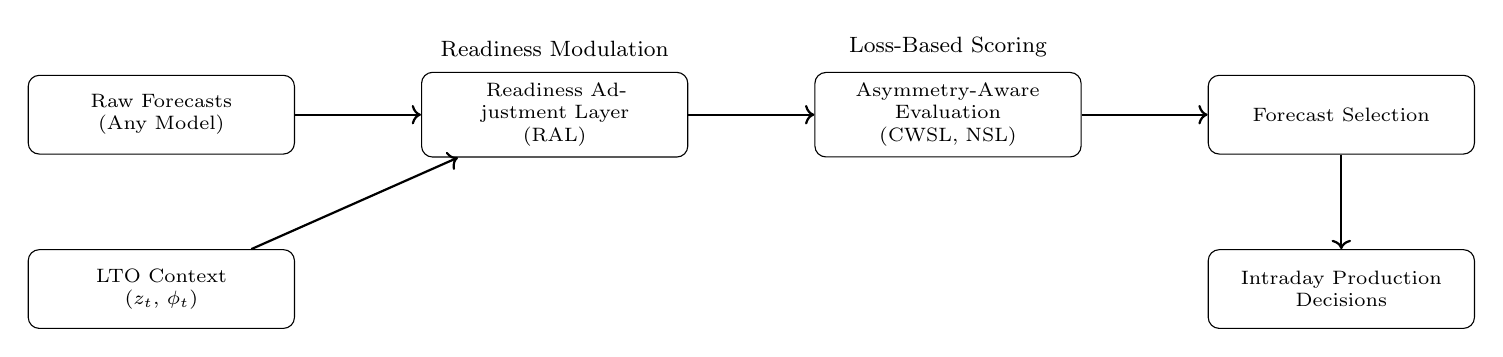
\begin{tikzpicture}[
    node distance=1.2cm and 1.6cm,
    font=\scriptsize,
    box/.style={
        draw,
        rectangle,
        rounded corners,
        align=center,
        text width=3.1cm,
        minimum height=1.0cm,
        inner sep=4pt
    },
    arrow/.style={->, thick}
]

% ----------------------------------------------------------
% NODES
% ----------------------------------------------------------

\node[box] (forecast) {Raw Forecasts\\(Any Model)};
\node[box, below=of forecast] (context) {\LTO{} Context\\(\ltoOn{}, \ltoPhase{})};

\node[box, right=of forecast] (ral) {Readiness Adjustment Layer\\(\RAL{})};
\node[box, right=of ral] (evaluation) {Asymmetry-Aware\\Evaluation\\(\CWSL{}, \NSL{})};
\node[box, right=of evaluation] (selection) {Forecast Selection};

\node[box, below=of selection] (production) {Intraday Production\\Decisions};

% ----------------------------------------------------------
% ARROWS
% ----------------------------------------------------------

\draw[arrow] (forecast) -- (ral);
\draw[arrow] (context) -- (ral);

\draw[arrow] (ral) -- (evaluation);
\draw[arrow] (evaluation) -- (selection);
\draw[arrow] (selection) -- (production);

% ----------------------------------------------------------
% ANNOTATIONS
% ----------------------------------------------------------

\node[above=2pt of ral] {\footnotesize Readiness Modulation};
\node[above=2pt of evaluation] {\footnotesize Loss-Based Scoring};

\end{tikzpicture}%
}

\caption{Readiness-centric production control under \LTO{} conditions in the Electric Barometer framework.
\LTO{} activation enters the system as contextual information that degrades forecast readiness via the
Readiness Adjustment Layer (\RAL{}), rather than as a demand uplift. Forecasts are evaluated under
asymmetry-aware loss and selected to minimize expected operational harm before being translated
into intraday production actions.}
\label{fig:lto-readiness-flow}
\end{figure}

\subsection{Purpose and positioning of the \RAL{}}
\label{subsec:ral-purpose}

Within the Electric Barometer architecture, \RAL{} sits between raw forecast generation and
readiness-aware evaluation. Its role is not to correct forecasts, improve accuracy, or estimate
demand uplift. Instead, it answers a narrower operational question:

\begin{quote}
\emph{Given current operating conditions, how much confidence should be placed in any forecast,
regardless of how it was produced?}
\end{quote}

This distinction is critical during \LTO{} periods. Forecasts may remain numerically reasonable yet
become operationally fragile due to increased variance, structural breaks, or execution
heterogeneity. \RAL{} captures this fragility explicitly, allowing downstream decision logic to
respond conservatively when trust is degraded.

\subsection{\LTOs{} as exogenous readiness shocks}
\label{subsec:lto-readiness-shocks}

As formalized in Section~\ref{sec:regime-shifts}, Electric Barometer treats \LTO{} activation as an
exogenous readiness shock. The presence of an active \LTO{} conveys reliable information about the
forecasting environment independent of any realized demand signal: uncertainty is elevated,
historical calibration is weakened, and the cost of error is likely to be asymmetric.

Formally, \LTO{} context enters the system through a binary or categorical indicator (e.g.,
\ltoOn{} or \ltoPhase{}), which is consumed by the \RAL{} rather than by the forecasting model
itself. This design ensures that the system responds to the \emph{existence} of planned instability
without embedding assumptions about its magnitude. Whether the promotion ultimately drives
substantial lift or negligible change, the readiness posture during the launch window reflects the
known increase in risk.

\subsection{Readiness modulation rather than demand adjustment}
\label{subsec:readiness-modulation}

A central design principle of \RAL{} is that readiness modulation is preferable to demand
adjustment under uncertainty. Adjusting demand forecasts upward to reflect expected \LTO{} lift
requires committing to a specific belief about future behavior; when that belief is wrong, the error
propagates directly into production decisions.

By contrast, readiness modulation alters how forecasts are evaluated and acted upon. Reduced
readiness during \LTO{} periods may manifest as increased tolerance for forecast dispersion,
heightened sensitivity to downside risk, or more conservative selection among candidate forecasts.
These responses increase preparedness without asserting that demand will increase by any
particular amount.

\subsection{Interaction with asymmetry-aware evaluation}
\label{subsec:ral-asymmetry}

The impact of \RAL{} is realized through its interaction with asymmetry-aware readiness primitives.
When readiness is reduced, downstream metrics such as \CWSL{} and \NSL{} exert greater influence
on forecast selection and decision support. In effect, \RAL{} amplifies the operational consequences
of error during high-risk periods without altering the underlying forecasts.

During hyped \LTO{} windows, this interaction biases production behavior toward shortfall
avoidance and service protection, particularly in peak dayparts. Importantly, this bias emerges from
governed loss asymmetry rather than from hard-coded demand uplift factors, preserving
explainability and auditability.

\subsection{Temporal dynamics of readiness}
\label{subsec:ral-temporal}

Readiness adjustment need not be static over the life of an \LTO{}. Launch, sustain, and wind-down
phases often exhibit distinct risk profiles. Early launch periods may warrant aggressive readiness
degradation due to uncertainty and execution variance, while later phases may allow partial
recovery as empirical demand signals accumulate.

The \RAL{} accommodates these dynamics by allowing readiness modulation to depend on phase-level
context (\ltoPhase{}) or elapsed time since activation. Such modulation remains rule-based and
transparent, avoiding adaptive behavior that could obscure governance or complicate postmortem
analysis.

\subsection{Role of \RAL{} in production management}
\label{subsec:ral-role}

By construction, \RAL{} does not attempt to predict demand, allocate inventory, or schedule
production. Its sole function is to ensure that forecast usage reflects the current risk environment.
In doing so, it enables Electric Barometer to operate effectively during periods when forecasts are
known \emph{ex ante} to be least reliable.

In the following section, we show how readiness-adjusted forecasts are evaluated and selected using
asymmetry-aware loss primitives, completing the mechanism by which \LTO{} context influences
intraday production decisions without relying on promotional demand models.
% ----------------------------------------------------------
% LOSS ASYMMETRY AND FORECAST SELECTION
% ----------------------------------------------------------

\section{Loss Asymmetry and Forecast Selection}
\label{sec:asymmetry}

Forecast selection in operational environments should reflect not only expected deviation from
realized demand, but the asymmetric consequences of being wrong. During \LTOs{}, these asymmetries
intensify: the cost of under-producing during peak promotional windows often exceeds the cost of
over-producing by a wide margin. Electric Barometer encodes this reality explicitly through
asymmetry-aware evaluation and selection, ensuring that production behavior aligns with operational
risk rather than numerical accuracy.

\subsection{Asymmetric loss as an operational primitive}
\label{subsec:asymmetric-loss}

Traditional accuracy metrics implicitly assume symmetry: over- and under-forecasting are penalized
equally. This assumption is rarely valid in production management, and it is especially brittle
during \LTO{} periods. Stockouts during promotional peaks can result in immediate revenue loss,
queue buildup, brand damage, and guest dissatisfaction, while moderate over-production may be
absorbed through holding buffers, reallocation, or controlled waste. Asymmetric loss has long been
recognized as essential for decision-aligned learning and evaluation \citep{elkan2001}.

Electric Barometer addresses this imbalance using asymmetric loss primitives, most notably
\CWSL{}. By weighting under-forecasting and over-forecasting differently via cost parameters
\cu{} and \co{}, \CWSL{} translates forecast error into an estimate of expected operational loss
rather than abstract deviation. This framing ensures that forecast evaluation is grounded in
decision consequence.

\subsection{Readiness-adjusted loss evaluation}
\label{subsec:readiness-adjusted-loss}

The influence of asymmetric loss is modulated by readiness. When the \RAL{} indicates degraded
readiness—such as during active \LTO{} launch phases—loss asymmetry becomes more decisive in
forecast selection. In effect, readiness adjustment amplifies the penalty associated with operationally
dangerous errors without altering the forecasts themselves.

Formally, readiness-adjusted evaluation can be viewed as applying asymmetric loss under a
context-dependent risk posture. Forecasts that appear similar under symmetric accuracy metrics
may diverge sharply once evaluated under \CWSL{} in a low-readiness environment. This divergence
guides Electric Barometer toward forecasts that better protect service and throughput during
high-risk periods.

\subsection{Selection over aggregation}
\label{subsec:selection-over-aggregation}

A key design choice in Electric Barometer is the emphasis on selection rather than aggregation.
Instead of averaging forecasts or blending models to improve point accuracy, the system evaluates
candidate forecasts under readiness-adjusted loss and selects the option that minimizes expected
operational harm.

This approach is particularly important during \LTO{} regimes, where averaging can dilute
protective bias and obscure downside risk. Selection preserves interpretability—each decision can
be traced to a specific forecast and evaluation context—and avoids overconfidence induced by
ensemble smoothing.

\subsection{Implications for production behavior}
\label{subsec:production-implications}

Asymmetry-aware selection produces concrete and intuitive effects on production behavior during
\LTO{} periods. Forecasts that err conservatively on the side of over-preparation are favored during
high-risk windows, increasing buffer availability and reducing the likelihood of service failure.
As uncertainty resolves and readiness recovers, selection pressure relaxes, allowing production to
tighten without abrupt regime changes.

Importantly, these effects arise without explicit demand uplift modeling. Production quantities
increase not because the system believes demand will be higher, but because the cost of being short
is higher. This distinction preserves robustness when promotional outcomes diverge from
expectations.

\subsection{Explainability and governance}
\label{subsec:asymmetry-governance}

Encoding asymmetry at the evaluation and selection stage improves explainability and governance.
Decisions can be justified in terms of explicit cost tradeoffs and readiness context rather than opaque
model internals. Postmortem analysis can distinguish between forecast misspecification and
appropriate risk posture, clarifying whether outcomes reflect modeling gaps or intentional
conservatism.

In the next section, we integrate readiness adjustment and asymmetric selection into an intraday
control loop, demonstrating how Electric Barometer operationalizes these principles in real-time
production management under \LTO{} conditions.
% ----------------------------------------------------------
% INTRADAY CONTROL LOOP
% ----------------------------------------------------------

\section{Intraday Control Loop}
\label{sec:intraday-loop}

Intraday production management is a closed-loop control problem. Decisions are made repeatedly
over short horizons, informed by realized demand signals and constrained by operational capacity.
Under \LTOs{}, this loop must operate in an environment of elevated uncertainty, where forecasts are
known to be less reliable but service risk is higher. Electric Barometer operationalizes readiness
adjustment and asymmetry-aware selection within a disciplined intraday control loop designed to
respond safely to unfolding conditions.

\subsection{Control loop structure}
\label{subsec:control-structure}

At each intraday decision point, the control loop proceeds through a fixed sequence:
\begin{enumerate}[leftmargin=*, itemsep=2pt]
  \item \textbf{Signal ingestion.} Observe realized sales velocity, queue conditions, and any
  relevant operational indicators available at time $t$.
  \item \textbf{Context evaluation.} Determine active contextual signals, including \LTO{}
  activation (\ltoOn{}) and phase (\ltoPhase{}), along with any binding capacity or supply
  constraints.
  \item \textbf{Readiness adjustment.} Apply the \RAL{} to modulate forecast trust based on the
  current context, yielding a readiness posture appropriate to the risk environment.
  \item \textbf{Forecast evaluation and selection.} Evaluate candidate forecasts under
  readiness-adjusted asymmetric loss (e.g., \CWSL{}), and select the forecast that minimizes
  expected operational loss.
  \item \textbf{Production action.} Translate the selected forecast into a production target
  \qprod{}, subject to feasibility and capacity constraints.
\end{enumerate}

This structure ensures that contextual risk influences decisions before production commitments are
made, while preserving a clear separation between observation, evaluation, and action.

\subsection{Role of realized demand}
\label{subsec:realized-demand}

Realized demand plays a central role in the intraday loop. As sales accumulate, uncertainty about
actual demand resolves naturally, reducing reliance on prior beliefs. Electric Barometer leverages
this resolution by allowing realized signals to dominate decision-making as the day progresses,
particularly during sustained \LTO{} periods.

Crucially, realized demand is not used to retroactively justify earlier assumptions about promotional
lift. Instead, it serves as a corrective signal that interacts with readiness and loss asymmetry to
update production behavior incrementally. This avoids abrupt shifts and reduces the risk of
overreaction to early noise.

\subsection{Partial reversibility and pacing}
\label{subsec:reversibility}

Intraday production decisions are partially reversible. Over-production can sometimes be mitigated
through holding buffers, reallocation across channels, or controlled waste, while under-production
during peak windows is often irreversible. Electric Barometer accounts for this asymmetry by
pacing production adjustments over time rather than committing to large, belief-driven jumps.

During \LTO{} launch phases, readiness-adjusted selection favors conservative ramps that protect
against shortfall. As empirical demand signals stabilize, production targets can be tightened
gradually, reflecting improved confidence without abandoning caution.

\subsection{Failure modes avoided}
\label{subsec:failure-modes}

The intraday control loop is explicitly designed to avoid common failure modes observed during
promotional periods:
\begin{enumerate}[leftmargin=*, itemsep=2pt]
  \item \textbf{Belief lock-in.} Production does not hinge on a single promotional lift estimate that
  must be defended throughout the day.
  \item \textbf{Overreaction to noise.} Early demand spikes do not immediately trigger aggressive
  scaling absent readiness-aware evaluation.
  \item \textbf{Delayed correction.} Conservative bias during high-risk windows reduces the
  likelihood of late-day stockouts that cannot be recovered.
\end{enumerate}

By structuring decisions around readiness and loss rather than point accuracy, Electric Barometer
maintains stability even when forecasts miss materially.

\subsection{Operational interpretability}
\label{subsec:intraday-interpretability}

An important property of the intraday control loop is interpretability. Each production decision can
be explained in terms of observable signals, contextual readiness, and explicit cost asymmetry.
Operators are not asked to trust opaque promotional models; instead, they are guided by a system
that behaves predictably under known risk conditions.

This interpretability supports operational adoption and governance, enabling teams to understand
why production was increased or constrained during \LTO{} periods. In the next section, we discuss
how these decisions are governed, monitored, and audited to ensure consistent behavior across
promotions and time.
% ----------------------------------------------------------
% GOVERNANCE AND REPORTING
% ----------------------------------------------------------

\section{Governance and Reporting}
\label{sec:governance}

Because \LTO{} periods deliberately alter risk posture and decision behavior, their integration into
production management must be governed explicitly. Without clear governance, readiness adjustment
and asymmetric selection risk being misinterpreted as ad hoc conservatism or model instability.
Electric Barometer therefore treats all readiness- and loss-related assumptions as first-class,
auditable artifacts rather than implicit system behavior.

\subsection{Governed contextual signals}
\label{subsec:governed-context}

All contextual signals that influence readiness must be declared, versioned, and inspectable. In the
case of \LTOs{}, this includes activation indicators (\ltoOn{}), phase labels (\ltoPhase{}), and any
rules governing their temporal extent. These signals define when and how readiness is degraded and
must be managed through the same governance processes as other operational parameters.

By externalizing \LTO{} context, Electric Barometer ensures that promotional effects are not
silently embedded in model behavior. This separation enables consistent application across stores,
dayparts, and promotions, and simplifies review when readiness assumptions change.

\subsection{Readiness policies and lifecycle}
\label{subsec:readiness-lifecycle}

Readiness adjustment policies should have an explicit lifecycle. The degree of readiness degradation
associated with \LTO{} launch, sustain, and wind-down phases must be specified in advance and
revisited periodically. Changes to these policies redefine operational risk posture and therefore
require review and approval. This emphasis on explicit assumptions and robustness over point
optimality aligns with established principles of sensitivity analysis and model governance
\citep{saltelli2008}.

Importantly, readiness policies are not tuned opportunistically in response to short-term outcomes.
They are calibrated based on historical behavior, operational tolerance, and governance objectives,
and then held fixed during evaluation and execution. This separation preserves interpretability and
prevents post hoc rationalization of performance.

\subsection{Loss asymmetry governance}
\label{subsec:loss-governance}

Asymmetric loss parameters (\cu{}, \co{}) encode explicit tradeoffs between service protection and
waste. During \LTO{} periods, these parameters often differ from steady-state values, reflecting the
heightened cost of shortfall. Because these weights directly influence production behavior, they must
be governed with the same rigor as readiness policies.

Governance artifacts should record the chosen cost ratios, their justification, and the contexts in
which they apply. This documentation enables postmortem analysis to distinguish between deliberate
risk posture and unintended consequences, and ensures that changes in loss asymmetry are deliberate
rather than emergent.

\subsection{Reporting and diagnostics}
\label{subsec:reporting-diagnostics}

Effective governance requires transparent reporting. For each \LTO{}, reporting should include:
\begin{enumerate}[leftmargin=*, itemsep=2pt]
  \item the period of \LTO{} activation and associated readiness posture,
  \item the loss asymmetry parameters applied during the promotion,
  \item summary diagnostics of forecast selection behavior under readiness adjustment, and
  \item observed service and waste outcomes relative to steady-state baselines.
\end{enumerate}

These diagnostics allow stakeholders to assess whether readiness adjustment and asymmetric
selection behaved as intended, independent of whether forecasts were numerically accurate.

\subsection{Postmortems and continuous improvement}
\label{subsec:postmortems}

Postmortem analysis under Electric Barometer focuses on decision quality rather than forecast error
alone. When outcomes deviate from expectations during \LTO{} periods, the primary questions are:
\begin{itemize}[leftmargin=*, itemsep=2pt]
  \item Were readiness policies appropriate given the risk environment?
  \item Were loss asymmetries aligned with operational priorities?
  \item Did the intraday control loop respond coherently to realized demand signals?
\end{itemize}

This framing avoids the reflexive conclusion that forecasting models must be improved whenever
outcomes are unfavorable. Instead, it supports targeted refinement of readiness and governance
assumptions, reinforcing the principle that operational robustness, not numerical accuracy, is the
ultimate objective.

In the next section, we examine common deployment patterns and failure modes observed when
managing \LTO{} periods, illustrating how the Electric Barometer approach differs from traditional
forecast-centric systems.
% ----------------------------------------------------------
% CASE PATTERNS AND FAILURE MODES
% ----------------------------------------------------------

\section{Case Patterns and Failure Modes}
\label{sec:patterns}

The abstract principles described in prior sections manifest in recognizable operational patterns
during \LTO{} deployments. Examining these patterns clarifies both the failure modes of traditional
forecast-centric systems and the stabilizing effects of a readiness-centric approach. This section
summarizes common behaviors observed in practice and situates Electric Barometer’s design choices
relative to these outcomes.

\subsection{Pattern 1: Belief-driven overcommitment}
\label{subsec:belief-overcommitment}

A frequent failure mode during \LTO{} launches is belief-driven overcommitment. In this pattern,
production plans are scaled aggressively based on a single promotional lift estimate, often derived
from historical analogs or marketing expectations. When realized demand underperforms these
assumptions, stores are left with excess production, elevated waste, and reduced flexibility for
later dayparts.

This failure mode arises from coupling production decisions directly to speculative demand beliefs.
Forecast accuracy metrics may indicate success \emph{ex ante}, yet operational outcomes deteriorate
when assumptions fail. Electric Barometer avoids this pattern by refusing to treat uplift estimates as
authoritative inputs to intraday control, instead favoring readiness-adjusted conservatism.

\subsection{Pattern 2: Accuracy chasing under instability}
\label{subsec:accuracy-chasing}

Another common pattern is reactive accuracy chasing. When early \LTO{} performance diverges from
expectations, forecasting systems are rapidly retuned or manually overridden in an attempt to
restore numerical accuracy. These interventions often lag realized demand and amplify volatility,
resulting in oscillatory production behavior.

Electric Barometer mitigates this failure mode by shifting the objective away from point accuracy.
Because readiness degradation is expected during \LTO{} regimes, forecast misses are not treated as
exceptions requiring immediate correction. Instead, asymmetric loss and readiness posture govern
selection, allowing production behavior to remain stable while uncertainty resolves naturally.

\subsection{Pattern 3: Late-day shortfall and irreversibility}
\label{subsec:late-day-shortfall}

A particularly costly failure mode occurs when conservative production early in the day is not
revisited under rising demand, leading to late-day shortfalls. In traditional systems, reluctance to
adjust forecasts upward without strong confidence can delay corrective action until it is too late to
recover service.

Under Electric Barometer, this pattern is addressed through the intraday control loop. Readiness
adjustment biases early decisions toward protection against shortfall, while continuous ingestion of
realized demand allows selection to shift as empirical evidence accumulates. This combination
reduces the likelihood of irreversible late-day service failures.

\subsection{Pattern 4: Postmortem misattribution}
\label{subsec:postmortem-misattribution}

Postmortems following \LTO{} underperformance frequently attribute poor outcomes to forecasting
inaccuracy alone. This narrow framing obscures whether decisions were reasonable given the risk
environment and often leads to unnecessary model complexity or ad hoc overrides in subsequent
promotions.

Electric Barometer reframes postmortems around decision quality. By making readiness posture and
loss asymmetry explicit, it becomes possible to assess whether outcomes reflected appropriate risk
management rather than predictive failure. This distinction supports more constructive learning and
avoids repeated cycles of reactive model tuning.

\subsection{Summary of contrasting behaviors}
\label{subsec:pattern-summary}

Table~\ref{tab:pattern-summary} summarizes the contrast between traditional forecast-centric
approaches and the readiness-centric patterns encouraged by Electric Barometer during \LTO{}
periods.

% ----------------------------------------------------------
% TABLE: Forecast-Centric vs Readiness-Centric Patterns
% ----------------------------------------------------------

\begin{table}[htbp]
\centering
\caption{Contrasting forecast-centric and readiness-centric operational patterns during \LTO{} periods}
\label{tab:pattern-summary}
\begin{tabular}{@{}p{4cm}p{5cm}p{5cm}@{}}
\toprule
\textbf{Aspect} & \textbf{Forecast-Centric Pattern} & \textbf{Readiness-Centric Pattern} \\
\midrule
Decision driver & Promotional lift belief & Readiness and loss asymmetry \\
Response to miss & Retune or override model & Maintain posture; adapt via signals \\
Early-day bias & Cautious until confident & Conservative against shortfall \\
Late-day recovery & Often delayed & Incremental and responsive \\
Postmortem focus & Accuracy failure & Decision alignment \\
\bottomrule
\end{tabular}
\end{table}

These patterns illustrate how Electric Barometer alters system behavior not by improving
predictive accuracy during \LTOs{}, but by changing how uncertainty is governed. The following
section discusses limitations and non-goals, clarifying the scope within which these design choices
are intended to operate.
\section{Limitations and Scope}

The Forecast Readiness Framework is intended as an evaluative structure for forecasting systems
operating under asymmetric error cost, and its applicability is subject to several limitations.
Recognizing these limitations clarifies the scope of the framework and helps avoid
misinterpretation of its intended use.

First, the framework depends on the specification of asymmetric penalty parameters, particularly
within the \CWSL\ component. These parameters encode the relative operational cost of shortfalls
and overbuilds and may vary across organizations, products, or decision contexts. While precise
monetary calibration is not required, poorly chosen penalty ratios may misrepresent true
operational priorities. In practice, sensitivity analysis and stakeholder input are necessary to
ensure that penalty structures reflect plausible asymmetry assumptions.

Second, the \FRF\ is designed for forecast evaluation rather than model training or optimization.
Although its diagnostics may inform modeling choices, the framework does not prescribe how
forecasts should be generated, nor does it guarantee optimal decisions when used as an
optimization objective. In particular, the composite \FRS\ is intended as a deployment and
governance signal, not as a loss function to be minimized during model fitting.

Third, the framework evaluates forecast performance conditional on realized demand and does
not explicitly account for uncertainty representation or probabilistic calibration. In environments
where full predictive distributions are available, readiness assessment may benefit from
complementary probabilistic diagnostics. The \FRF\ does not replace such approaches but
addresses a distinct evaluative need centered on operational execution and asymmetric cost.

Finally, the framework abstracts from certain system-level constraints, such as downstream
dependencies, dynamic feedback effects, or capacity interactions across items or locations. While
the diagnostic dimensions capture important aspects of readiness at the forecast level, additional
analysis may be required to assess system-wide performance in highly coupled operational
settings.

These limitations reflect deliberate design choices rather than deficiencies. By focusing on
deployment readiness under asymmetric error structures, the \FRF\ addresses a specific gap in
forecast evaluation while remaining compatible with broader modeling and decision-support
approaches.
\section{Conclusion}

Forecasts used in operational decision-making are ultimately judged not by numerical accuracy
alone, but by their ability to support reliable execution under asymmetric cost. In many applied
settings, traditional symmetric accuracy metrics fail to capture the directional, temporal, and
economic structure of forecast error that determines operational success or failure. As a result,
forecasts that appear accurate by conventional measures may still impose unacceptable service
risk when deployed.

This paper introduced the \emph{Forecast Readiness Framework} (\FRF) as a structured approach
for evaluating forecast performance in such environments. By decomposing readiness into
complementary dimensions—service reliability, failure severity, tolerance stability, and economic
consequence—the framework provides a diagnostic lens that extends beyond aggregate accuracy.
Within this structure, Cost-Weighted Service Loss (\CWSL) serves as the economic axis, translating
directional forecast error into cost-aligned impact, while supporting diagnostics reveal how error
patterns affect execution.

The framework further incorporates a composite readiness signal, the \FRS, to support
deployment-level decisions, monitoring, and governance. Rather than collapsing evaluation into a
single loss function, the \FRF\ preserves interpretability while enabling principled trade-offs between
efficiency and reliability. Through an illustrative example, the paper demonstrated how forecasts
with comparable symmetric accuracy can exhibit sharply different readiness profiles, underscoring
the limitations of conventional evaluation practices.

By reframing forecast evaluation around readiness for deployment under explicit and governed
assumptions, the \FRF\ provides a practical and generalizable basis for assessing forecasting
systems in asymmetric operational contexts. Sensitivity analysis, calibration procedures, and
policy-based constraints ensure that readiness assessments are transparent, auditable, and stable
across models and time periods. More broadly, the framework encourages a shift in forecast
evaluation from measuring how close predictions are to realized demand toward understanding
how forecast error shapes operational outcomes in practice.


% ==========================================================
% REFERENCES
% ==========================================================
\bibliographystyle{plainnat}
\bibliography{references}

\end{document}
